\documentclass[a4paper]{article}
% same but with two columns
%\documentclass[a4paper,twocolumn]{article}

\usepackage{amsmath}                    % for equation, align
\usepackage{amsthm}                     % for theorem
%\usepackage[titletoc,title]{appendix}   % support 'appendices' section with proper names
\usepackage[english]{babel}             % for different language support
\usepackage{booktabs}                   % for beautiful tables
\usepackage{csvsimple}                  % for csv tables
\usepackage{empheq}                     % for boxed equations
\usepackage{float}                      % for H option in figures to put them in same place as in text
\usepackage{graphicx}                   % for figures
\usepackage{hyperref}                   % required for \href
\usepackage{lipsum}                     % for example text
%\usepackage[nottoc,numbib]{tocbibind}   % include references to the table of contents
\usepackage[nottoc]{tocbibind}          % same but do not add a number to the `References` entry
\usepackage{subcaption}                 % for subfigures
\usepackage{todonotes}                  % keep track of todo items during writing
\usepackage{url}                        % for \url
\usepackage{vhistory}                   % for revision history

% define environment `theorem` and name every according one `Theorem` in text
\newtheorem*{theorem}{Theorem}

\begin{document}

\title{How losses outweight gains: study of a simple price oscillation case}
\author{Viktors Boroviks, \href{mailto:vboroviks@inbox.lv}{vboroviks@inbox.lv}}
\date{\vhCurrentDate, v\vhCurrentVersion}
\maketitle

% enable page numbering and set current page to 1 after the title
\pagenumbering{arabic}
\setcounter{page}{1}

\begin{abstract}

Following two major cases are studied:

\begin{enumerate}
\item price change by the same absolute amount --- gains required to cover equivalent loss,
\item price change by the same relative amount --- total loss resulting from oscillation of price.
\end{enumerate}

Simple equations are provided as well as reference tables, example figures
and suggestions for gain/loss management.

\end{abstract}

%commented out as standard structure is used
%\tableofcontents

\section*{Disclaimer}

While looking through related literature I failed to find the description
of this simple yet frequently overlooked phenomenon from the mathematical
point of view.

As a result --- terminology and conclusions listed are of my own.
Corrections are welcome.

\section*{Introduction}

Usually, when asymmetry of gains and losses is discussed --- it is viewed
as a psychological phenomenon of risk aversion.

My focus in this article is instead on the underlying simple mathematics.

When the price rises and falls on a certain asset --- intuitively we assume
that if such change happened for the same relative amount, say 10\% increase
followed by 10\% decrease --- we would end up in the same starting position.
But in reality, we end up at a loss.

The following is true:

\begin{theorem}
Subsequent change in price in opposite directions
can be equal either by the absolute amount
or relative amount (percentage), but not both.
\end{theorem}

\begin{theorem}
When comaring the result of price increase and decrease by the same relative
amount --- losses always overweight equivalent gains.
\end{theorem}

\section*{Generic case}

Generic case considered in this article can be described as price change
between three points $P_1$, $P_2$ and $P_3$:

\begin{equation}
  \begin{cases}
    P_1 \xrightarrow{d_{12}} P_2 \xrightarrow{d_{23}} P_3,\\
    P_1 \xrightarrow{d_{13}} P_3
  \end{cases}
\end{equation}

where $d_{12}$, $d_{23}$, $d_{13}$ --- price deviation from 1.

\begin{equation}
  (1 + d_{12}) \dot (1 + d_{23}) = 1 + d_{13}
\end{equation}

$d$ variables are not absolute, but have direction defined by its sign.
Gains are positive and losses are negative.

Price deviation could be defined from prices:

\begin{subequations}
\begin{align}
  \frac{P_2}{P_1} = 1 + d_{12}; \ \Rightarrow \ &d_{12} = \frac{P_2}{P_1} - 1,\\
                                                &d_{23} = \frac{P_3}{P_2} - 1,\\
                                                &d_{13} = \frac{P_3}{P_1} - 1
\end{align}
\label{eq:p1_p2_p3}
\end{subequations}

Two significant corner cases exist and are described in following sections.

\section*{Price change by the same absolute amount}

The price changes from $P_1$ to $P_2$
and then returns to the original level.
See the Figure~\ref{fig:diag_p1_p2} below.

\begin{equation}
  \begin{cases}
    P_1 \xrightarrow{d_{12}} P_2 \xrightarrow{d_{23}} P_3,\\
    P_1 \xrightarrow{d_{13}} P_3,\\
    (1 + d_{12}) \dot (1 + d_{23}) = 1 + d_{13},\\
    P_1 = P_3 \ \Rightarrow \ \begin{cases}
                                d_{13} = 0,\\
                                d_{21} := d_{23}
                              \end{cases}
  \end{cases}
  \Rightarrow
  \begin{cases}
    P_1 \xrightarrow{d_{12}} P_2 \xrightarrow{d_{21}} P_1,\\
    (1 + d_{12}) \dot (1 + d_{21}) = 1.
  \end{cases}
\end{equation}

\begin{figure}[H]  % H = insert picture precisely here
\centering
\hfill  % move pictures apart at equal distance
\subcaptionbox{Price rises and falls.}
  [0.4\textwidth]{\includegraphics{diag_p1_p2_inc.pdf}}
\hfill
\subcaptionbox{Price falls and rises.}
  [0.4\textwidth]{\includegraphics{diag_p1_p2_dec.pdf}}
\caption{Cases for price change by the same absolute amount.}%
\hfill
\label{fig:diag_p1_p2}
\end{figure}

Price deviation defined from prices, based on the Equation~\ref{eq:p1_p2_p3}:

\begin{empheq}[box=\fbox]{align}
  d_{12} = \frac{P_2}{P_1} - 1,
  \quad  % horizontal space between equations: https://www.overleaf.com/learn/latex/Spacing_in_math_mode
  d_{21} = \frac{P_1}{P_2} - 1
\end{empheq}

Price deviation defined from other deviation:

\begin{empheq}[box=\fbox]{align}
  d_{12} = \frac{1}{1 + d_{21}} - 1,
  \quad  % horizontal space between equations: https://www.overleaf.com/learn/latex/Spacing_in_math_mode
  d_{21} = \frac{1}{1 + d_{12}} - 1
\label{eq:p1_p2_d21}
\end{empheq}

Practical application for trading is suggested in Conclusions.

\subsection*{Examples}

Following examples demonstrate how bigger losses require exponentially greater
gains to return to the original position.

If up to $1\%$ this effect is negligible, then after loss of $80 \dots 90\%$
practical recovery becomes close to impossible.

\begin{table}[H]
  \centering
  \csvautobooktabular[respect all]{abs_change.csv}
  \caption{Equivalent gains and losses if price oscilates by the same absolute amount.}
  \label{tab:abs_change}
\end{table}

\begin{figure}[H]  % H = insert picture precisely here
\centering
\hfill  % move pictures apart at equal distance
\subcaptionbox{Losses up to 20\%.}
  [0.4\textwidth]{\includegraphics{abs_change_rate1.pdf}}
\hfill
\subcaptionbox{Losses up to 99\%.}
  [0.4\textwidth]{\includegraphics{abs_change_rate2.pdf}}
\hfill
\caption{Gains required to break even after a loss. Red line shows 1-to-1 Gain/Loss ratio.}
\label{fig:abs_change}
\end{figure}

\section*{Price change by the same relative amount}

The price changes from $P_1$ to $P_2$ to $P_3$, but it is known that
the price deviation is the same in both cases.
and then returns to the original level.
See the Figure~\ref{fig:diag_p1_p2_p3} below.

\begin{equation}
  \begin{cases}
    P_1 \xrightarrow{d_{12}} P_2 \xrightarrow{d_{23}} P_3,\\
    P_1 \xrightarrow{d_{13}} P_3,\\
    d_{12} = -d_{23} \ \Rightarrow \ \begin{cases}
                                       d_{13} \ne 0,\\
                                       P_1 \ne P_2 \ne P_3.
                                     \end{cases}
  \end{cases}
\end{equation}

\begin{figure}[H]  % H = insert picture precisely here
\centering
\hfill  % move pictures apart at equal distance
\subcaptionbox{Price rises and falls.}
  [0.4\textwidth]{\includegraphics{diag_p1_p2_p3_dec.pdf}}
\hfill
\subcaptionbox{Price falls and rises.}
  [0.4\textwidth]{\includegraphics{diag_p1_p2_p3_inc.pdf}}
\hfill
\caption{Cases for price change by the same relative amount.}
\label{fig:diag_p1_p2_p3}
\end{figure}

Price deviation defined from prices is the same as in
the Equation~\ref{eq:p1_p2_p3}.

Price deviation defined from other deviation:

\begin{align}
  \begin{cases}
  d_{12} = -d_{23},\\
  (1 + d_{12})(1 + d_{23}) = 1 + d_{13}
  \end{cases}
  \Rightarrow
  \begin{cases}
    d_{12} = -d_{23},\\
    \boxed{d_{13} = -d_{12}^2 = -d_{23}^2}
  \end{cases}
  \label{eq:p1_p2_p3_d13}
\end{align}

Practical application for trading is suggested in Conclusions.

\subsection*{Examples}

In the Table~\ref{tab:rel_change} we can see, that price oscillation by the
same relative value brings exponentially bigger losses, the bigger is the
oscillation amplitude.

This is a counter-intuitive effect, where we would expect no change to
the total price after oscillation.

\begin{table}[H]
  \centering
  \csvautobooktabular[respect all]{rel_change.csv}
  \caption{Total losses if price oscilates by the same relative value.}
  \label{tab:rel_change}
\end{table}

\begin{figure}[H]  % H = insert picture precisely here
\centering
\hfill  % move pictures apart at equal distance
\subcaptionbox{Losses up to 1\%.}
  [0.4\textwidth]{\includegraphics{rel_change_rate1.pdf}}
\hfill
\subcaptionbox{Losses up to 100\%.}
  [0.4\textwidth]{\includegraphics{rel_change_rate2.pdf}}
\hfill
\caption{Total losses if price oscilates by the same relative value.}
\label{fig:rel_change}
\end{figure}

Figure~\ref{fig:rel_change} demonstrates no difference to the resulting price
if oscillaiton begins with the price increase or decrease.

As expected, such effect would result in accumulating losses over longer
period.

\begin{figure}[H]  % H = insert picture precisely here
\centering
\hfill  % move pictures apart at equal distance
\subcaptionbox{Price increases then falls.}
  [0.4\textwidth]{\includegraphics{rel_osc_inc.pdf}}
\hfill
\subcaptionbox{Price falls then increases.}
  [0.4\textwidth]{\includegraphics{rel_osc_dec.pdf}}
\hfill

\subcaptionbox{Oscillation over longer period.}
  {\includegraphics[width=\textwidth]{rel_osc_inc_n150.pdf}}
\caption{Oscillations of price by 10\% at every iteration.}
\label{fig:rel_change}
\end{figure}

\section*{Conclusions}

When tracking relative price change, to not end up in a loss,
ensure (from the Equation~\ref{eq:p1_p2_d21}):

\begin{subequations}
\begin{empheq}[box=\fbox]{align}
  d_{rise} \ge \frac{1}{1 - \left|d_{previous\ fall}\right|} - 1,\\
  \left|d_{fall}\right| \le \left|\frac{1}{1 + d_{previous\ rise}} - 1 \right|
\end{empheq}
\end{subequations}

It is wise to control losses.
As seen from the examples provided in this article, gains required to
break even after a loss grow exponentially, eventually culminating in such
catastrophic losses that recovery from them becomes practically impossible.

Also, if you had a price change sequence for the same relative amount,
you would always end up at a loss equal to:

\begin{empheq}[box=\fbox]{align}
  d_{loss} = -d_{rise}^2 = -d_{fall}^2
\end{empheq}

The loss grows exponentially relative to the oscillation amplitude.

There is no differene if price first rises or falls (see Equation~\ref{eq:p1_p2_p3_d13}).

As a result, after a period of trading with equal relative gains and losses
you would end up at a growing total loss, the longer the trading period and
the bigger the price oscillation amplitude.

% appendices
% start from a new page
\clearpage
\section*{Appendix}

All source files for this article available at:

\begin{itemize}
\item \url{https://github.com/viktorsboroviks/viktorsboroviks.github.io}
\item tag: v1.0
\end{itemize}

% disable page numbering for the revision history page
\pagenumbering{gobble}

% version history
% switching to onecolumn is required if the document is forwmatted as twocolumn
\begin{onecolumn}

\begin{versionhistory}
\vhEntry{1.0}{19 Feb 2023}{VB}{Initial version.}
\end{versionhistory}

\end{onecolumn}

\end{document}
